\documentclass{article}
\usepackage[T1]{fontenc}
\usepackage[utf8]{inputenc}
\usepackage[romanian]{babel}
\usepackage{amsmath}
\usepackage{tikz}
\usetikzlibrary{angles,quotes}
\usepackage[european]{circuitikz}
\usepackage{pgfplots}
\pgfplotsset{compat=1.18}
\usepackage[margin=2cm]{geometry}
\author{Neacșu Andrei}
\title{Întrebări și răspunsuri \\ Electricitate}
\newcounter{question}
\setcounter{question}{0}

\newcommand{\question}[1]{\item[\textbf{Î.\refstepcounter{question}\thequestion.}] \textit{#1}}
\newcommand{\answer}[1]{\item[R.\thequestion.] #1}

\begin{document}
\maketitle
    \begin{itemize}
    
            \question{ Care este structura internă a electronului? Care este structura internă a protonului?
Cât este valoarea sarcinii electrice a unui electron? Cât este masa unui electron? Cât
este valoarea spinului electronului și ce semnificație are această valoare?}

            \answer{Electronul este considerat o particulă elementară, deci \textbf{nu are o structură internă}, nu se poate „desface” în ceva mai mic. Spre deosebire de electron, protonul \textbf{are o structură internă complexă}. \textbf{Este format} din quarci (doi up și unul down), care sunt ținuți împreună de particule purtătoare de forță numite gluoni. \textbf{Valoarea sarcinii electrice} a unui electron este $q_e \approx -1.602 \cdot 10^{-19} ~ \text{coulombi (C)}$. \textbf{Masa unui electron} este $ m_e \approx 9.109 \cdot 10^{-31} ~ kg$. \textbf{Valoarea spinului electronului} este $s=\frac{1}{2}$ și reprezintă o proprietate cuantică intrinsecă, un fel de "moment cinetic" pe care particula îl are pur și simplu, fără să se rotească fizic în spațiu. Deoarece are spin semi-întreg, electronul este un fermion, însemnând că respectă \textit{Principiul de excluziune al lui Pauli} (doi electroni nu pot ocupa aceeași stare cuantică simultan în atom.)} 
            
            
            \question{ Ce este sarcina electrică? Ce înseamnă că sarcina electrică este o mărime cuantificată?}
            
            \answer{\textbf{Sarcina electrică} este o proprietate fundamentală a particulelor subatomice care determină interacțiunile electromagnetice ale acestora. Faptul că sarcina este \textit{cuantificată} înseamnă că ea nu poate avea orice valoare, ci există doar ca un multiplu întreg al unei valori minime, numită sarcină elementară $e \approx 1,602 \cdot 10^{-19} ~ C$. Astfel, orice sarcină electrică $Q$ din univers respectă relația $Q = n \cdot e$, unde $n$ este un număr întreg.}
            
            
            
            \question{Cum a fost măsurată sarcina electrică a electronului de către Millikan? Cum a fost determinată masa
electronului?}

            \answer{Sarcina electrică a electronului a fost determinată prin celebrul \textit{experiment al picăturii de ulei} realizat de Robert Millikan în 1909. Metoda s-a bazat pe pulverizarea unor picături fine de ulei într-o cameră etanșă, unde acestea se încărcau electrostatic prin frecare. Millikan a lăsat picăturile să cadă sub influența gravitației pentru a le determina masa, iar apoi a aplicat un câmp electric vertical între două plăci metalice.Echilibrând forța gravitațională ($F_g = m \cdot g$) cu forța electrică ($F_e = q \cdot E$), Millikan a reușit să facă anumite picături să „plutească” nemișcate. Din condiția de echilibru $qE = mg$, el a calculat sarcina $q$ pentru mii de picături diferite. Rezultatele au arătat că sarcina era întotdeauna un multiplu întreg al unei valori minime, $e \approx 1,602 \cdot 10^{-19} ~ C$, demonstrând astfel că sarcina este cuantificată. Masa electronului ($m_e$) nu a fost măsurată direct în acest experiment, ci a fost dedusă matematic. J.J. Thomson măsurase anterior, folosind tuburi cu raze catodice, raportul specific sarcină/masă al electronului, notat cu $e/m_e$. Odată ce valoarea precisă a lui $e$ a fost stabilită de Millikan, masa a fost calculată.}
            
            
            
         \question{Ce este interacțiunea electrostatică? Explicați legea Coulomb pentru interacțiunea dintre două sarcini electrice.}
         
         \answer{Interacțiunea electrostatică este forța de atracție sau de respingere care apare între corpuri aflate în stare de repaus, posesoare de sarcină electrică. Această interacțiune este guvernată de \textit{Legea lui Coulomb}, care stabilește că forța electrostatică ($F$) dintre două sarcini punctiforme este direct proporțională cu produsul modulelor celor două sarcini ($q_1, q_2$) și invers proporțională cu pătratul distanței ($r$) dintre ele. Matematic, legea se exprimă prin formula:$$ F = k \cdot \frac{|q_1 \cdot q_2|}{r^2} $$unde $k$ este o constantă de proporționalitate numită constanta electrostatică.}
         
         
         
         \question{Ce este curentul electric? Care este formula intensității curentului electric? Explicați printr-un exemplu numeric diferența dintre un curent electric mai intens și unul mai puțin intens.}
         
         \answer{Curentul electric reprezintă mișcarea ordonată a purtătorilor de sarcină electrică printr-un mediu conductor, iar mărimea fizică ce măsoară acest flux se numește intensitate ($I$), fiind definită de raportul $I = \Delta Q / \Delta t$. Unitatea de măsură este Amperul (A), ce corespunde trecerii unei sarcini de un coulomb pe secundă; spre exemplu, dacă într-un interval de $2~s$ secțiunea unui conductor este traversată de o sarcină de $10~C$, intensitatea curentului este de $5~A$, în timp ce o sarcină de doar $2~C$ în același interval indică un curent mai puțin intens, de $1~A$. Din punct de vedere calitativ, un curent mai intens reprezintă un transport mai mare de sarcină electrică în unitatea de timp, fiind analog cu un debit mai mare de apă printr-o conductă unde o cantitate mai mare de fluid tranzitează secțiunea tubului în același interval de timp.}
         
         
         
         \question{În graficul intensitatea curentului electric în funcție de timp, în cazul în care curentul este constant în timp, ce semnifică aria de sub graficul curentului? Dar dacă curentul crește liniar în timp?}
         
         \answer{În ambele cazuri, aria de sub grafic reprezintă sarcina electrică totală ($\Delta Q$) transportată prin conductor. Justificarea se bazează pe faptul că aria unei figuri geometrice se obține prin produsul dimensiunilor de pe cele două axe; în acest grafic, axa verticală reprezintă intensitatea ($I = \Delta Q / \Delta t$), iar axa orizontală timpul ($\Delta t$). Înmulțind cele două mărimi, timpul se simplifică, rămânând doar sarcina electrică ($I \cdot \Delta t = \Delta Q$).}
         
         
         
         \question{Ce înseamnă un curent de intensitate electrică $1 \, Amper$?}
         
		 \answer{Un curent de $1~A$ reprezintă o sarcină electrică de $1~C$ care trece prin secțiunea unui conductor în fiecare secundă. De exemplu, dacă un dispozitiv funcționează cu un curent de $1 ~ A$ timp de un singur minut, prin el vor circula $60 ~ C$ de electricitate, deci peste $300$ de miliarde de miliarde de electroni.}
		 
		 
		 
		 \question{Câți electroni se mișcă într-o secundă prin secțiunea firului, dacă intensitatea curentului este de $1 ~ A$?}
		 
		 \answer{Prin definiție, o intensitate $I = 1 ~ A$ corespunde unei sarcini $\Delta Q = 1 ~ C$ ce traversează secțiunea conductorului în intervalul $\Delta t = 1 ~ s$. $$ I = \frac{\Delta Q}{\Delta t} \Rightarrow \Delta Q = I \cdot \Delta t = 1 ~ A \cdot 1 ~ s = 1 ~ C $$Deoarece sarcina totală este formată dintr-un număr întreg $n$ de sarcini elementare $e$, avem:$$ n = \frac{\Delta Q}{e} = \frac{1 ~ C}{1,602 \cdot 10^{-19} ~ C} \approx  \boxed{6,242 \cdot 10^{18} \text{ electroni}} $$}
		 
		 
		 
	     \question{Scrieți legea lui Ohm. Numiți mărimile din lege și unitățile lor de măsură. Explicați legea electric și printr-o analogie neelectrică din natură.}
	     
	     \answer{$U=I \cdot R$, unde $U$ este căderea de tensiune, măsurată în volți (V), $I$ este intensitatea curentului electric, măsurată în amperi (A) și $R$ este rezistența electrică, măsurată în ohmi($\Omega$). Într-un conductor, electronii se mișcă haotic; pentru a crea un curent, avem nevoie de o „motivație” exterioară. Tensiunea ($U$) este cea care creează un câmp electric ce forțează electronii să se deplaseze într-o direcție precisă. Totuși, aceștia nu pot accelera la infinit deoarece se ciocnesc constant de atomii conductorului, iar această opoziție este rezistența ($R$). Intensitatea ($I$) reprezintă fluxul de sarcini care „supraviețuiește” acestor ciocniri sub acțiunea tensiunii. Dacă dublăm tensiunea, dublăm forța care acționează asupra fiecărui electron, deci fluxul (intensitatea) se va dubla, presupunând că structura materialului (rezistența) rămâne neschimbată. Un exemplu din natură este un râu care curge prin munți. Tensiunea ($U$) este analoagă cu gravitația care împinge apa la vale. Cu cât muntele este mai abrupt, cu atât apa are mai multă „tensiune”. Intensitatea($I$) este debitul apei. Rezistența ($R$) este reprezentată de bolovanii și îngustările din albia râului care încetinesc cursul apei. Dacă albia este plină de bolovani mari (rezistență mare), debitul apei va fi mic, chiar dacă panta muntelui este mare.}
	     
	     
	    
	  		 
         \question{Dacă o rezistență electrică este supusă pe rând la trei curenți $I_1, I_2, I_3$ și au loc astfel căderile de tensiuni electrice $U_1, U_2, U_3$, ce relație matematică se poate scrie între aceste intensități și tensiuni? Cum arată graficul tensiunii electrice în funcție de intensitate?}
         
         \answer{Deoarece rezistența $R$ a conductorului este constantă, conform legii lui Ohm, raportul dintre tensiune și intensitate se menține invariant. Relația matematică este:$$\frac{U_1}{I_1} = \frac{U_2}{I_2} = \frac{U_3}{I_3} = R = \text{const.}$$Graficul tensiunii în funcție de intensitate este o dreaptă care trece prin originea sistemului de axe: \begin{center}
\begin{tikzpicture}
\begin{axis}[
axis lines = middle,
xlabel = {$I$},
ylabel = {$U$},
xmin=0, xmax=4,
ymin=0, ymax=4,
xtick={1,2,3},
ytick={1,2,3},
xticklabels={$I_1$, $I_2$, $I_3$},
yticklabels={$U_1$, $U_2$, $U_3$},
width=8cm, height=6cm
]
% Desenăm dreapta
\addplot [domain=0:3.5, color=blue, thick] {x};

\addplot[only marks, mark=*] coordinates {(1,1) (2,2) (3,3)};
\coordinate (D) at (0,0);
\draw[dashed] (1,1) coordinate (C) -- (0,1) coordinate (B);
\draw[dashed] (C) -- (1,0) coordinate(A);
\draw[dashed] (2,2) -- (2,0);
\draw[dashed] (2,2) -- (0,2);
\draw[dashed] (3,3) -- (3,0);
\draw[dashed] (3,3) -- (0,3);
\draw pic [draw,->,black,thick,"$\theta$", angle radius=1cm] {angle = A--D--C};
\end{axis}
\end{tikzpicture}\\
Graficul Tensiunii în funcție de Intensitate
\end{center}
 Panta dreptei reprezintă valoarea rezistenței electrice $\left(R= \tan \theta = \frac{U_1}{I_1}\right)$. O pantă mai mare indică o rezistență mai ridicată, deoarece este necesară o tensiune mai mare pentru a menține același flux de curent.}
 
 
 		         \question{Scrieți trei formule pentru rezistența electrică. Numiți situația în care se folosește fiecare formulă.}
 		         
 		         \answer{Rezistența electrică se calculează diferit în funcție de datele disponibile:
\begin{itemize}
    \item[$\bullet$] $R = \frac{U}{I}$ -- \textbf{Legea lui Ohm}: utilizată în analiza circuitelor. 
    \item[$\bullet$] $R = \rho \frac{L}{S}$ -- \textbf{Formula constructivă}: utilizată pentru a determina rezistența în funcție de materialul și dimensiunile geometrice ale firului. $\rho$ reprezintă rezistivitatea materialului, $L$ lungimea firului și $S$ aria secțiunii.
    \item[$\bullet$] $R = R_0(1 + \alpha \Delta t)$ -- \textbf{Dependența termică}: utilizată pentru a calcula variația rezistenței unui conductor în funcție de temperatura acestuia. $R_0$ este rezistența la $0^\circ C$, $\alpha$ coeficientul termic de rezistivitate al materialului și $\Delta t$ variația temperaturii.
\end{itemize}}


				\question{Explicați cum variază rezistența odată cu lungimea și odată cu secțiunea.}
				
				\answer{Dacă lungimea ($L$) crește, rezistența ($R$) crește. Dacă secțiunea ($S$) crește, rezistența ($R$) scade.}
				
				
				
				\question{Scrieți valorile pentru rezistivitatea electrică a materialului a cinci materiale diferite, unitatea de măsură în sistem internațional și institutele de la care ați luat valorile.}
				\answer{ Unitatea de măsură în SI pentru rezistivitatea electrică a unui material este ohm-metru ($\Omega \cdot m$).

\begin{table}[h]
    \centering
    \begin{tabular}{|l|c|l|}
        \hline
        \textbf{Material} & \textbf{Rezistivitate} ($\Omega \cdot m$ la $20^\circ C$) & \textbf{Sursa / Institutul} \\ \hline
        Argint  & $1,59 \cdot 10^{-8}$ & NIST (SUA) \\ \hline
        Cupru   & $1,68 \cdot 10^{-8}$ & NIST \\ \hline
        Aur     & $2,44 \cdot 10^{-8}$ & NIST \\ \hline
        Aluminiu & $2,82 \cdot 10^{-8}$ & NIST \\ \hline
        Tungsten (Wolfram) & $5,60 \cdot 10^{-8}$ & IUPAC / NIST \\ \hline
    \end{tabular}
    \caption{Valorile rezistivității electrice pentru materiale conductoare.}
\end{table}} 
         
         
         \question{Scrieți formula de variație a rezistenței odată cu temperatura și explicați termenul adițional pe care aceasta îl dobândește prin încălzire.}
         
         \answer{Formula de variație a rezistenței este: $R = R_0 + R_0\alpha \Delta t$. Pe măsură ce temperatura crește, ionii din rețeaua cristalină a metalului vibrează mult mai intens în jurul pozițiilor lor de echilibru. Aceste vibrații termice măresc „haosul” din interiorul conductorului, ceea ce face ca electronii să se ciocnească mult mai des de ioni în drumul lor.}
         \newpage
         
         \question{Scrieți valorile pentru coeficientul termic de rezistivitate $\alpha$ a materialului a cinci materiale diferite, unitatea de măsură în sistem internațional și institutele de la care ați luat valorile.}
				\answer{ Unitatea de măsură în SI pentru coeficientul termic de rezistivitate electrică a unui material este $^\circ C^{-1}$. 
				\begin{table}[h]
\centering
\begin{tabular}{|l|c|l|}
\hline
\textbf{Material} & \textbf{Valoare} $\alpha$ ($^\circ C^{-1}$) & \textbf{Sursa / Institutul} \\ \hline
Argint & $0,0038$ & NIST \\ \hline
Cupru (călit) & $0,00393$ & NIST \\ \hline
Aluminiu & $0,00429$ & HyperPhysics (GSU) \\ \hline
Wolfram (Tungsten) & $0,0045$ & CRC Handbook of Physics \\ \hline
Fier & $0,00651$ & HyperPhysics (GSU) / NIST \\ \hline
\end{tabular}
\caption{Coeficienți termici de rezistivitate pentru materiale metalice.}
\end{table}}


			\question{Desenați un circuit simplu și scrieți-i elementele.}
			\answer{\begin{itemize}
    \item[$\bullet$] \textbf{Generatorul (Sursa):} Dispozitivul care produce și menține curentul electric în circuit (ex: bateria). Caracterizat prin tensiunea electromotoare $E$ și rezistența internă $r$.
    \item[$\bullet$] \textbf{Consumatorul:} Dispozitivul care transformă energia electrică în altă formă de energie (ex: rezistorul). Caracterizat prin rezistența $R$.
    \item[$\bullet$] \textbf{Conductoarele de legătură:} Fire care fac legătura între sursă și consumator.
\end{itemize} 
{\centering
\begin{circuitikz}
  \draw
  (0,2) to[battery1, l={{$E, r$}}] (2,2)
  (2,2) to[short] (2,0)
  (2,0) to[R, l=$R$] (0,0)
  (0,0) to[short] (0,2);
\end{circuitikz}\\Figura 1: Circuitul simplu\par}}
			
			
			\question{Scrieți enunțul legii a doua a lui Kirchhoff pentru un ochi de rețea.}
			\answer{Pe un ochi de circuit, suma algebrică a tensiunilor electromotoare ($E$) este egală cu suma algebrică a căderilor de tensiune ($I \cdot R$) de pe fiecare ramură.}
			
			\question{Scrieți legea a doua a lui Kirchhoff pentru circuitul simplu și numiți mărimile fizice.}
			\answer{$ E= U+u$, unde:
			\begin{itemize}
			\item[$\bullet$] $E$ reprezintă tensiunea electromotoare;
			\item[$\bullet$] $U$ reprezintă tensiunea la bornele bateriei;
			\item[$\bullet$] $u$ reprezintă tensiunea electrică internă;
			\end{itemize}}
			
			
			\question{Scrieți bilanțul în tensiuni, puteri și energii în circuitul electric simplu.}
			\answer{Bilanț în tensiuni: $E = U + u $\\
			Bilanț în puteri: $EI = UI + uI$\\
			Bilanț în energii: $EIt = UIt + uIt$}
			
			
			\question{Scrieți bilanțul în tensiuni, puteri și energii în circuitul electric simplu și numiți tensiunile, puterile și energiile.}
			\answer{

     Bilanțul tensiunilor: $E = U + u$
    \\ ($E$ – t.e.m., $U$ – tensiune la borne, $u$ – cădere de tensiune internă)\\
    Bilanțul puterilor: $EI = UI + uI$
    \\ ($EI$ – puterea totală, $UI$ – puterea utilă, $uI$ – puterea disipată intern)\\
    Bilanțul energiilor: $EIt = UIt + uIt$
    \\ ($EIt$ – energia furnizată, $UIt$ – energia utilă, $uIt$ – energia pierdută)

}

			\question{Scrieți formula puterii electrice în mai multe forme în funcție de tensiune și curent. Justificați când este utilă fiecare formă.}
			\answer{$P=UI=I^2R=\frac{U^2}{R}$\\Alegem forma în funcție de datele cunoscute sau datele invariabile (ex. circuite în serie, $I = const.$)}
			
			\question{Scrieți formula intensității curentului electric în circuitul simplu.}
			\answer{$I=\frac{E}{R+r}$}
			
			\question{Schițați bilanțul energiilor electrice în circuit. Deduceți formula randamentului circuitului simplu.}
			\answer{Randamentul circuitului simplu: $\eta = \frac{W_{util}}{W_{total}} = \frac{UIt}{EIt} = \frac{U}{E} = \frac{RI}{RI+rI} = \frac{R}{R+r}$
			\begin{center}
			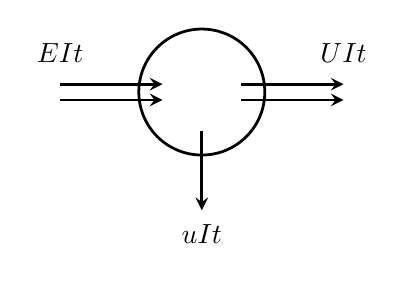
\begin{tikzpicture}[line width=1pt, >=stealth]
   	 \draw (0,0) circle (0.8cm);
   	 \draw[->] (-1.8, 0.1) -- (-0.5, 0.1);
   	 \draw[->] (-1.8, -0.1) -- (-0.5, -0.1);
   	 \node at (-1.8, 0.5) {$EIt$};
   	 \draw[->] (0.5, 0.1) -- (1.8, 0.1);
   	 \draw[->] (0.5, -0.1) -- (1.8, -0.1);
   	 \node at (1.8, 0.5) {$UIt$};
   	 \draw[->] (0, -0.5) -- (0, -1.5);
   	 \node at (0, -1.8) {$uIt$};
\end{tikzpicture}\\
Figura 2: Bilanțul energiilor electrice \end{center}}

			\question{Scrieți valoarea rezistenței echivalente a două rezistențe electrice legate în serie și în paralel.}
			\answer{$\boxed{R_s = R_1 +R_2}$\\ $\frac{1}{R_p} = \frac{1}{R_1}+\frac{1}{R_2} = \frac{R_1+R_2}{R_1R_2} \Rightarrow \boxed{R_p = \frac{R_1R_2}{R_1+R_2}}$}
			
			\question{Când este intensitatea electrică mai mare în circuitul simplu, când două rezistențe electrice sunt legate în serie sau în paralel la sursă?}
			\answer{
    Intensitatea este mai mare în \textbf{paralel}. 
    \\ \textbf{Justificare:} Rezistența echivalentă în paralel ($R_p$) este întotdeauna mai mică decât cea în serie ($R_s$). Conform legii lui Ohm $I = \frac{E}{R+r}$, cu cât rezistența exterioară este mai mică, cu atât intensitatea curentului este mai mare:
    $$R_p < R_s \implies \boxed{ I_{paralel} >  I_{serie}}$$
}

			\question{Descrieți structura internă a unei baterii obișnuite din comerț.}
			\answer{O baterie obișnuită (celulă galvanică) este formată dintr-un înveliș exterior de zinc care servește drept anod (pol negativ). În centrul acestuia se află o tijă de grafit, care joacă rolul de catod (pol pozitiv) și este înconjurată de un amestec de dioxid de mangan și pudră de cărbune. Spațiul dintre cei doi electrozi este umplut cu un electrolit sub formă de pastă (de obicei clorură de amoniu sau hidroxid de potasiu), care facilitează reacțiile chimice necesare producerii curentului electric.}
			
			\question{Descrieți pilele Volta.}
			\answer{Pila Volta, inventată de Alessandro Volta în anul 1799, reprezintă prima sursă de curent electric continuu din istorie. Aceasta a demonstrat că electricitatea poate fi generată pe cale chimică. Pila este formată dintr-o coloană (stivă) de elemente care se repetă, perechi de discuri metalice din metale diferite, de regulă zinc (anod - polul negativ) și cupru sau argint (catod - polul pozitiv). Între perechile de discuri se află un strat de material poros (carton sau hârtie) îmbibat într-o soluție acidă sau salină (apă sărată sau acid sulfuric diluat. Funcționarea se bazează pe reacții de oxidoreducere: \\
			La Anod (Zinc): Atomii de zinc se oxidează și trec în soluție sub formă de ioni pozitivi ($Zn^{2+}$), eliberând electroni în circuitul exterior.\\
			La Catod (Cupru): Ionii de hidrogen din electrolit acceptă electronii veniți prin circuit și se transformă în bule de gaz (hidrogen). Cuprul are rolul de conductor, nefiind consumat în reacție.\\
			 Dezavantaje: Bulele de hidrogen care se formează pe discul de cupru creează un strat izolator, ceea ce duce la scăderea rapidă a intensității curentului; Un singur element generează o tensiune foarte mică, motiv pentru care trebuie suprapuse foarte multe discuri (de unde și denumirea de „pilă”).}
			 
			 \question{Scrieți valoarea tensiunii electromotoare echivalente și rezistența electrică internă echivalentă în locul a două surse electrice în serie.}
			 \answer{$E_s = E_1 + E_2$ \\ $r_s = r_1 + r_2$}
			 
			 \question{Scrieți valoarea tensiunii electromotoare echivalente și rezistența electrică internă echivalentă în locul a două surse electrice în paralel.}
			 \answer{$E_p= \frac{E_1r_2+E_2r_1}{r_1+r_2}$\\
			  $r_p = \frac{r_1r_2}{r_1+r_2}$}
			 
			 \question{Ce înseamnă circuit în gol? Dar scurtcircuit?}
			 \answer{Circuitul în gol reprezintă situația când circuitul este deschis, nu există consumator (Intensitatea $I$ este 0 și tensiunea $U$ este tensiunea electromotoare). Scurtcircuitul se produce în situația când bornele sursei sunt conectate între ele printr-un conductor cu rezistența zero ($R = 0$). Intensitatea $I_{sc}$ este egală cu $  \frac{E}{r}$ și tensiunea $U$ este nulă.} 
			 
			 \question{Analizați matematic situația montării unei rezistențe care scade de la infinit la zero în circuitul exterior. Analizați tensiunea la bornele rezistenței. Analizați intesitatea în circuitul simplu.}
			 \answer{Orice sursă de tensiune continuă (baterie, acumulator) prezintă în interiorul său o rezistență proprie numită rezistență internă ($r$). Din acest motiv, tensiunea măsurată la bornele sursei în timp ce aceasta debitează curent este mai mică decât tensiunea sa nominală (tensiunea electromotoare, $E$).Montajul experimental (Figura 3) este conceput pentru a varia intensitatea curentului din circuit prin intermediul unui reostat ($R$). Pe măsură ce cursorul reostatului este deplasat, rezistența exterioară se modifică, permițând înregistrarea mai multor perechi de valori $(I, U)$ cu ajutorul voltmetrului și ampermetrului. Funcționarea circuitului este guvernată de Legea lui Ohm pentru întregul circuit:$$I = \frac{E}{R + r}$$Din această relație putem deduce ecuația caracteristicii externe, care exprimă tensiunea la borne ($U = I \cdot R$) în funcție de intensitatea curentului ($I$):$$E = I \cdot R + I \cdot r \implies U = E - I \cdot r$$ Această ecuație este de tipul $y = mx + n$ (unde $m = -r$ și $n = E$), reprezentând matematic o funcție liniară descrescătoare. Graficul obținut prin trasarea dreptei de ecuație menționată anterior evidențiază regimurile de funcționare ale sursei: 
			 \begin{itemize}
			 \item[$\bullet$] Mersul în gol ($R \to \infty$): Când circuitul este deschis, intensitatea curentului este nulă ($I = 0$). În acest punct, căderea de tensiune internă dispare ($I \cdot r = 0$), iar voltmetrul indică valoarea maximă: $\mathbf{U = E}$. 
			\item[$\bullet$]  Regimul normal: În regim normal, rezistența consumatorului $R$ are o valoare finită ($R \in (0, \infty)$). Tensiunea are valoarea $\mathbf{U = E - I \cdot r}$.
			\item[$\bullet$]  Regimul de scurtcircuit ($R = 0$): Când bornele sursei sunt unite printr-un fir fără rezistență, tensiunea la borne devine nulă ($\mathbf{U = 0}$). Curentul atinge valoarea maximă: $\mathbf{I_{sc} = \frac{E}{r}}$.
			\end{itemize}
			 \begin{minipage}{0.45\textwidth}
			 \begin{center}
			 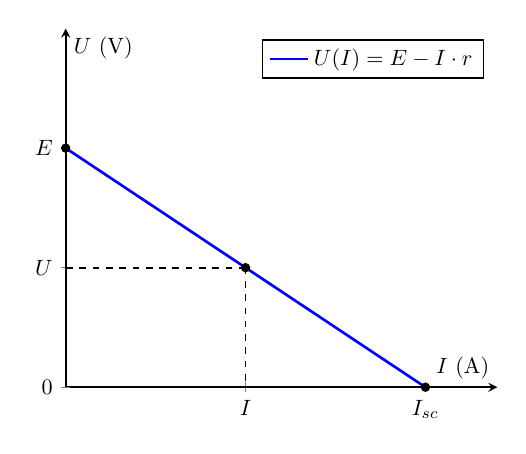
\begin{tikzpicture}[scale=0.8]
\begin{axis}[
    axis lines = middle,
    xlabel = {$I$ (A)},
	ylabel = {$U$ (V)},
    ymin = 0, ymax = 1.5,
    xmin = 0, xmax = 1.2,
    xtick = {0.5, 1},
    xticklabels = { $I$, $I_{sc}$},
    ytick = {0, 0.5, 1},
    yticklabels = {0, $U$, $E$},
    extra y ticks={0},
    extra y tick labels={0},
    legend pos = north east,
    grid = none,
    clip = false,
    thick
]
    \addplot [
        domain=0:1, 
        samples=2, 
        color=blue,
        very thick,
    ]
    {1 - x};
	\addlegendentry{$U(I) = E - I \cdot r$}
	\draw [dashed] (0.5, 0.5) -- (0.5, 0);
	\draw [dashed] (0.5, 0.5) -- (0, 0.5);
    \node[circle, fill, inner sep=1.5pt] at (axis cs:0,1) {};
    \node[circle, fill, inner sep=1.5pt] at (axis cs:0.5,0.5) {};
    \node[circle, fill, inner sep=1.5pt] at (axis cs:1,0) {};
    
   
\end{axis}
\end{tikzpicture}\\Graficul Tensiunii în funcție de Intensitate când rezistența scade \end{center} \end{minipage}
\hfill
\begin{minipage}{0.45\textwidth}
\begin{center}
\begin{circuitikz} [scale = 0.8, transform shape]
    \draw (0,0) 
    to[battery1, l={{$E, r$}} ] (0,3)
    to[ammeter, l=$I$] (3,3)           % Ampermetru sau fir
    to[vR, l_=$R$] (3,0)              % Rezistor variabil (Reostat)
    to[short] (0,0);                 % Închidere circuit
    
    % Voltmetru în paralel cu R
    \draw (3,3) -- (4,3) to[voltmeter, l=$U$] (4,0) -- (3,0);
\end{circuitikz} \\ Figura 3: Montaj experimental\end{center}\end{minipage}}

			\question{ Scrieți parametrii electrici ai unui încărcător de telefon. Explicați, comparați din punct de vedere electric mai multe tipuri de încărcător.}
			\answer{\textbf{Parametrii electrici principali:}
Orice încărcător (sursă de tensiune stabilizată) este definit de:
\begin{itemize}
    \item \textbf{Tensiunea nominală ($U$):} Standard $5\text{V}$ DC. Cele moderne (Fast Charge) pot urca la $9\text{V}$, $12\text{V}$ sau $20\text{V}$.
    \item \textbf{Curentul maxim ($I_{max}$):} Capacitatea debitată (ex: $1\text{A}$, $2.1\text{A}$, $3\text{A}$).
    \item \textbf{Puterea ($P$):} Produsul $U \cdot I$. Un încărcător de $20\text{W}$ livrează energie mult mai rapid decât unul de $5\text{W}$.
\end{itemize}



\begin{table}[h]
\centering
\begin{tabular}{|l|c|c|c|l|}
\hline
\textbf{Tip Încărcător} & \textbf{Tensiune} & \textbf{Curent} & \textbf{Putere nominală} & \textbf{Efect Electric} \\ \hline
Standard & $5\text{V}$ & $1\text{A}$ & $5\text{W}$ & Randament scăzut, încălzire la folosire. \\ \hline
Fast Charge (QC) & $9\text{V}$ & $2\text{A}$ & $18 \text{W}$ & Putere mare prin creșterea $U$ \\ \hline
GaN (Modern) & $20\text{V}$ & $5\text{A}$ & $100 \text{W}$ & Rezistență internă $r$ minimă, eficiență mare. \\ \hline
\end{tabular}
\caption{Compararea mai multor tipuri de încărcătoare}
\end{table}

\textbf{Concluzie fizică:}
Din punct de vedere al caracteristicii $U(I) = E - Ir$, un încărcător performant are o \textbf{rezistență internă ($r$) extrem de mică}. Acest lucru permite ca, deși curentul $I$ crește semnificativ pentru a încărca bateria repede, tensiunea $U$ să rămână stabilă, minimizând energia pierdută sub formă de căldură în adaptor.
}

			\question{Scrieți parametrii electrici ai unui server, ai unei surse PC, ai unei mașini de spălat, ai unui uscător de păr.}
			\answer{Parametrii se regăsesc în tabela de mai jos: \begin{table}[h]
\centering
\begin{tabular}{|l|c|c|c|}
\hline
\textbf{Consumator} & \textbf{U (V)}  & \textbf{I (A)} & \textbf{Putere Nominală (W)} \\ \hline
Server & 230  & 2.6 & 600  \\ \hline
Sursă PC & 230  & 3.2  & 750  \\ \hline
Fier de călcat & 230  & 10.4  & 2400  \\ \hline
Mașină de spălat & 230  & 9.5  & 2200  \\ \hline
Uscător de păr & 230  & 7.8  & 1800 \\ \hline
\end{tabular}
\caption{Parametrii electrici ai unor dispozitive}
\end{table}
	}
			\question{Care este standardul de tensiune electrică la priză în România? Dar în alte țări? Descrieți un adaptor pentru altă țară și numiți, din punct de vedere electric, diferența dintre standarde.}
			\answer{\begin{itemize}
    \item[$\star$] \textbf{România și majoritatea țărilor:} $U = 230 \pm 10\% \, \text{V}$, $f = 50 \, \text{Hz}$.
    \item[$\star$] \textbf{SUA, Canada:} $U = 120 \, \text{V}$, $f = 60 \, \text{Hz}$.
\end{itemize}

\textbf{Diferența electrică:} Un adaptor de priză realizează doar o \textit{conexiune mecanică}. Din punct de vedere electric, dacă tensiunile diferă, este necesar un \textbf{transformator} sau un \textbf{convertor}, nu doar un adaptor. Dispozitivele marcate cu "INPUT: 100-240V" sunt singurele care pot folosi adaptoare simple fără riscul de a se defecta.}
          \end{itemize}

\end{document}
